% This is samplepaper.tex, a sample chapter demonstrating the
% LLNCS macro package for Springer Computer Science proceedings;
% Version 2.20 of 2017/10/04
%
\documentclass[runningheads]{llncs}
%
\usepackage{graphicx}
\usepackage{amssymb}
% Used for displaying a sample figure. If possible, figure files should
% be included in EPS format.
%
% If you use the hyperref package, please uncomment the following line
% to display URLs in blue roman font according to Springer's eBook style:
% \renewcommand\UrlFont{\color{blue}\rmfamily}

\begin{document}
%
\title{Coordinate Matrix Machine: An Augmented Intelligence Approach to Classify Very Similar Documents}
\titlerunning{Coordinate Matrix Machine}
%
%\titlerunning{Abbreviated paper title}
% If the paper title is too long for the running head, you can set
% an abbreviated paper title here
%
\author{Amin Sadri \and
M. Maruf Hossain\thanks{corresponding author}}
%
\authorrunning{Sadri and Hossain}
% First names are abbreviated in the running head.
% If there are more than two authors, 'et al.' is used.
%
\institute{Australia and New Zealand Banking Corporation\\
\email{\{sadria,maruf.hossain\}@anz.com}\\
\url{http://www.anz.com/}}
%
\maketitle              % typeset the header of the contribution
%
\begin{abstract}
Document classification, in general, focuses primarily on the context of the document and classify based on its belonging to one or more classes. However, if the documents are more structured and contains very similar content to one another, then traditional approaches do not yield the required high accuracy demanded by many applications.

\textbf{Contribution.} In this paper, we have proposed a coordinate matrix-based approach which augments human intelligence to create a very small vector to learn the structure of the document and use this information to classify the documents.

\textbf{Result.} The algorithm outperforms every popular vectoriser techniques in combination with traditional machine learning and most advanced deep learning models that rely on a larger number of elements to achieve good accuracy. The advantages of our algorithm are:
\begin{enumerate}
\item Better accuracy
\item Faster computation
\item Small memory footprint
\item Generic, expandable and extendable
\item Explainable
\item Robust against unbalanced classes
\item Does not require large number of labelled data
\end{enumerate}

\keywords{Augmented intelligence \and Coordinate Matrix \and Lazy Learning \and Classification.}
\end{abstract}

%
%
\section{Introduction}
Human-level concept learning is a relatively newer area of research. The goal is to provide a solution to a problem that is easy for human to do, yet still hard for machines despite of their computational power. People can learn new concepts easily from only one or very few samples, while machine learning methods needs plenty of example to find correlations and understand features. The reason is that people subconsciously pick the important features and then generalise to other distinct areas~\cite{lake2015,mnih2015}.

In this paper, we deploy a human-level concept learning approach for document classification. Document classification is a common task in machine learning in the form of Natural Language Processing (NLP) where a document is assigned to one or more classes. Current approaches rely heavily on the context of the document in order to classify them~\cite{jones1972,power2010}. Identifying the relevant topic is the primary motivator for such document classification~\cite{hassan2017,kotenko2015,lin2006}. These models assume we have access to plenty of labelled data and the context of the documents are enough informative to distinguish between classes. Some other methods use the image information of the documents which makes the labelling process even worse. As an image is a high dimensional data, we need to label so many training samples that is not doable in most of the problems in reality~\cite{krizhevsky2012}.

A practical situation would be, when bank statements from other financial institutions are received along with loan applications, the task falls on to identify the templates for those statements so that existing functions can be applied to extract information from those statements. In reality, when we ask someone to classify these statements, we do not need to show them hundreds of samples for each class. Just one sample is enough for presenting one class. This fact shows us one sample is informative enough for classification if the algorithm is well-designed. This is our motivation for developing our algorithm. 

\textit{Our aim is to improve the classification performance on high number of classes by incorporating domain knowledge, i.e., augmenting human intelligence, when there is very small training data and the documents are very similar to one another.}

\subsection{Challenges}
When there is a large variation of structured documents that needs to be classified based on the structure of the document, machine learning techniques tends to suffer from poor performance. We have identified the following challenges when dealing with bank statements in particular:
\begin{itemize}
\item A large number of documents need to be labelled to train a model with sufficient accuracy, which is both time and resource consuming.
\item There are way too many class labels at the template level. For the five banks included in this experiment, there were 53 templates (classes) available. There are not enough representative samples for each class.
\item All bank statements look very similar to one another as all of them include many transaction descriptions, dates, and amounts.
\item Majority of the words in bank statements are personal and highly contextual, such as account holder's name, address or transaction items, which produces lots of noise when training a classification model.
\item The words which are not noise are very similar across a range of bank statements, e.g., ‘Name’, ‘Account’, ‘Balance’, ‘Date’.
\end{itemize}

Due to these challenges, traditional machine learning models and more recent deep learning models do not perform well. 
\begin{example}
While classifying statements using Term Frequency Vectoriser with Logistic Regression, the model with the best possible parameters yielded an $F$-measure of 79\% when we attempted to classify the templates. 
\end{example}

This lower performance can discourage users to use simplistic models and inclined to use more complex models like Convolutional Neural Network (CNN) or Recurrent Neural Network (RNN) \cite{banerjee2019,kumar2019}, which are by default not explainable, and rely on additional techniques~\cite{ribeiro2016} to explain, especially to the governing body for compliance purpose.
\begin{example}
After running hours to build CNN or Long Short-Term Memory (LSTM) RNN architecture, we have found that CNN could yield a $F$-measure of 93\%, but LSTM failed to classify 53 templates.
\end{example}

\subsection{Our Contribution}
In this paper, we apply a human-level concept learning~\cite{lake2015} to address this problem. We choose this approach because as a human we do not need hundreds of training samples to learn one class, and we are able to classify the documents even when the content are similar, sometimes even without reading the texts. Only one sample per template is enough and we should consider not only the content but also the location of certain words.

The closest work to our work in terms of the nature of the approach is the research conducted by Lake et al.~\cite{lake2015}. They have argued that in most cases people can learn a new concept from just one or a handful of examples, while typical machine learning algorithms require hundreds of examples to perform similarly. They aim towards a different problem and recognise every handwritten characters from image data. While in this paper, we aim to classify structured documents from text data. Although the problems are different, both works use human-level concept learning by looking at the way a human solve the problem. Both approaches only use one sample per class and learn from that sample.

Given documents of similar structure, as human we look at the structure of the document and/or the position of some keywords (e.g., Account Name, Date, Bank Name etc.). Similarly, in our approach, we have proposed a hybrid lazy learning algorithm, Coordinate Matrix Machine (CM$^2$), to create an input matrix (which contrasts with traditional vector-based input strategy) containing the coordinates for the keywords and use this matrix to classify documents.

The rationale behind the technique are as follows:
\begin{enumerate}
\item With structured documents, the position carries more importance than the occurrence or the order of the occurrence for the terms. Furthermore, by augmenting the understanding of the subject matter experts, we can avoid developing huge corpus, thus remove noises and eventually improve classification performance.
\item This technique would allow us to avoid labelling large amount of documents often needed to train machine learning and deep learning models.
\end{enumerate}

\subsection{Advantages}
The advantages of our algorithm are:
\begin{enumerate}
\item It has better accuracy compared to all algorithms tested.
\item It has faster computation.
\item It is generic, expandable and extendable. For newer samples, there is no need for any feature engineering or feature extraction.
\item It is explainable. It is easy to trace the reason behind classification and modify, if necessary. 
\item It is not affected by unbalanced classes, low-volume or low-quality training data.
\item It does not require large number of labelled data.
\end{enumerate}

\subsection{Organisation}
The remainder of the paper is organised as follows. In Section~\ref{work}, we briefly discuss the related work in document classification. Our algorithm is formally described in Section~\ref{algo}. Section~\ref{exp} presents the design of the experimental investigation. We present and discuss the results in Section~\ref{result} and~\ref{discuss}. Finally, in Section~\ref{conc}, we suggest future improvements and conclude the paper.

\section{Related Work}\label{work}
As document classification has become an emerging area in the text mining research, a large amount of prior work has focused on it. A typical document classification has several pre-processing steps and researches focused on each step to improve the performance, such as stopwords removal~\cite{manalu2017,prathibha2015}, Tokenization~\cite{bakar2014,gadri2015}, Part-of-Speech Tagging~\cite{owoputi2012}, Stemming~\cite{zhang2007}.

The second step usually focus on feature extraction and selection. For example, Yang et al.~\cite{yang2002} used titles and other tag data to label the text features. Shih and Karger~\cite{shih2004} used the geometry of the rendered HTML page to build up tree models based on the incoming link structure. Term Frequency–Inverse Document Frequency (TF-IDF) is a popular way for feature selection~\cite{jones1972}. Power et al.~\cite{power2010} focused on web page classification and filtered the output of the TF-IDF algorithm to improve the performance.

Once the feature vector is identified, the third step is to apply a machine learning model for classification. Na\"ive Bayes is one of the probability-based classifiers~\cite{kotenko2015}. Decision tree-based approaches have also been used for different purposes such as inappropriate web content blocking~\cite{liu2017}. Support Vector Machines (SVM) are also widely used for document classification~\cite{farhoodi2010,lin2006}. There are multiple approaches under artificial/deep neural network. Hassan and Mahmood~\cite{hassan2017} applied Convolution Neural Networks (CNN) for document classification. Unlike most of the machine learning models, Recurrent Neural Networks (RNN) take the sequence of the occurrences of the words into consideration, therefore documents with similar words will have different outputs because of the order of the words~\cite{banerjee2019,kumar2019}.

\section{Methodology}\label{algo}
We now describe in more detail, the steps in our algorithm for creating the coordinate matrix and inducing the classifier using the matrix.

\subsection{Pre-processing the Documents}
Each training data is a PDF file contains either a scanned image or a digital document. We have ensured that each page of the document is set to 300 dpi before we run the pages through an Optical Character Reader (OCR) engine to get the words and their respective coordinates. The output of the OCR is stored as eXtensible Mark-up Language (XML) files that are used as input to induce our model.

\subsection{Building the Coordinate Matrix}
For each class, only one sample is required for training. We accompany a Comma Separated Value (CSV) file with each XML file, which contains key-value pair for all keywords within the document.
\begin{example}
Statement A contains the term `Account No.’ followed by the account number `061234-12345678’, the term `Account Holder’ with the value `John Doe’, and the term `Account Type’ with the value `Savings Account’. Whereas, in statement B, the relevant term `Account No.’ followed by the number `064321-87654321’, and the term `Account Name’ with the value `Jane Smith’ is recorded. So in the CSV file for statement A, we have the entries ``\texttt{Account No.,061234-12345678}'', ``\texttt{Account Holder,John Doe}'' and ``\texttt{Account Type,Savings Account}''; and for statement B, we have ``\texttt{Account No.,064321-87654321}'' and ``\texttt{Account Name,Jane Smith}'' recorded. We then search for the keywords (e.g., `Account No.', `Account Name') in the XML file and construct a matrix with top and left position for each keyword for each document as shown in Tab.~\ref{matrix}.
\end{example}
\begin{table}[t]
\centering
\caption{Example of the Coordinate Matrix}\label{matrix}
\begin{tabular}{llrr}
\toprule
Document ID & Keyword & Top & Left\\
\midrule
Statement A & Account No. & 254 & 1231\\
Statement A & Account Holder & 261 & 1231\\
Statement A & Account Type & 269 & 1231\\
Statement B & Account No. & 1123 & 231\\
Statement B & Account Name & 100 & 359\\
\bottomrule
\end{tabular}
\end{table}

The first column comes from the training data, the second column comes from the CSV file accompanied with each XML file, and the last two columns are the search result for the keywords in the XML files. Algorithm~\ref{ccm} lists the steps.
\IncMargin{1.5em}
\begin{algorithm}[b!]
\SetKwData{CM}{$\mathcal{CM}$}
\SetKwData{counter}{$row$}
\SetKwFunction{GetCoordinates}{GetCoordinates}
\SetKwInOut{Input}{Input}
\SetKwInOut{Output}{Output}
\SetKw{Return}{return}
\Input{$\mathcal{T}= \{t_1, t_2, \ldots, t_N\}$, where $t_i$ is a training sample of $i^{th}$ class and $N$ is the total number of class.\newline
$\mathcal{K}=\{K_1, K_2, \ldots, K_N\}$, where $K_i = \{k^i_1, k^i_2, \ldots k^i_{M_i}\}$ is a set of keywords for $i^{th}$ class, $k^i_j$ is the $j^{th}$ keyword of $i^{th}$ class, and $M_i$ is the total number of the keywords for $i^{th}$ class.}
\Output{\CM: Matrix of coordinates for all keywords for all training samples, i.e., $\langle t_i, k^i_j, x_{ij}, y_{ij} \rangle$ for every $1 \leqslant i \leqslant N$, $1 \leqslant j \leqslant M_i$}
\BlankLine
\Begin{
$M \leftarrow \sum_{i=1}^{N} M_i$\tcp*[r]{total number of keywords}
$\counter \leftarrow 1$\;
$\CM \leftarrow M \times 4$ matrix\;
\For{$i \leftarrow 1$ to $N$}{
	\For{$j \leftarrow 1$ to $M_i$}{
		$\langle x_{ij}, y_{ij} \rangle \leftarrow \GetCoordinates(t_i, k^i_j)$\;
		$\CM_{\counter} \leftarrow \langle t_i, k^i_j, x_{ij}, y_{ij} \rangle$\;
		$\counter \leftarrow \counter + 1$\;
	}
}
\Return $\CM$\;
}
\BlankLine
\BlankLine
\tcp{Function to get the coordinates of a keyword}
\Fn{\GetCoordinates{$\mathcal{D}$, $k$}}{
\Input{$\mathcal{D}$: a document as XML\newline
$k$: the keyword to find in the document.}
\Output{$\langle x, y \rangle$: the coordinates of the start position of the keyword $k$ in the document $\mathcal{D}$.}
\BlankLine
\If{$k \in \mathcal{D}$}{
\Return $\langle x, y \rangle$ \tcp*[r]{the keyword is found}
}
\Return $\varnothing$\;
}
\caption{Build the Coordinate Matrix\label{ccm}}
\end{algorithm}
\DecMargin{1.5em}

\subsection{Classifying New Documents}
When a new document comes in, we run OCR on the documents. On the XML produced by the OCR, we look for all the words in the test document. We do this to ensure the approach stays robust against rotation or shift of the coordinates that can occur during the document scanning process.

We match the extracted words against all the keywords on the training data. Once we extract the matched keywords, we then form a coordinate matrix for the test cases comprising the top and left position. 
\begin{example}
Test case contains the term `Account No.’ followed by the account number `061111-11111111’, and the term `Account Name’ with the value `Jane Doe’. So the coordinate matrix for the test case would be as shown in Tab.~\ref{matrix2}. The second column in the table includes all the keywords available in the training coordinate matrix.
\end{example}
\begin{table}[tb]
\centering
\caption{Coordinate Matrix for the Test Case}\label{matrix2}
\begin{tabular}{llrr}
\toprule
Document ID & Keyword & Top & Left\\
\midrule
Test case & Account No. & 1120 & 230\\
Test case & Account Holder & -- & --\\
Test case & Account Type & -- & --\\
Test case & Account Name & 101 & 360\\
\bottomrule
\end{tabular}
\end{table}

We then calculate the distance for each keyword between the test data vs every training sample. To calculate the distance between the keywords, Manhattan distance has been used. We used Manhattan distance because it gives less value to the horizontal and vertical shifts compared to the diagonal shifts. The horizontal and vertical shifts is more likely in a document due to extra empty line or space.

We have introduced only one parameter in this algorithm.
\begin{definition}
\textbf{Maximum Penalty} is the maximum distance allowed between two keywords. If the distance between the same keywords from two documents is more than this threshold, then the actual distance is substituted by this value. Besides, when a keyword is not found in a document the distance for that keyword is set to this value. In other word, if the distance between the keyword found and its counterpart is more than the \textbf{maximum penalty}, we assume that keyword is not found in the document.
\end{definition}

We defined this parameter for two reasons:
\begin{enumerate}
\item There should be a distance value even when we cannot locate a keyword in a document otherwise we cannot apply the mean function in the next step.
\item We want to ensure that the algorithm is robust by limiting the effect of a single keyword. Otherwise, if a keyword in two documents is very far, either due to the poor extraction quality of the OCR or being a variant of the training data, the calculated distance will be too great.
%We want to ensure that the algorithm is robust. A few mismatched keywords, either due to the poor extraction quality of the OCR or being a variant of the trained template, between documents do not have any greater effect on the overall similarity calculation. Otherwise, if a keyword in two documents is very far, or if similar set of words is picked up by mistake, the defined distance will be too high.
\end{enumerate}

Finally, we calculate the mean distance for all keywords of each training sample to get a similarity score between the test case and that training sample. The sample that has the minimum distance to the test case identifies the class. Algorithm~\ref{classify} lists the steps and Example~\ref{example} demonstrates the calculation.
\IncMargin{1.5em}
\begin{algorithm}[t!]
\SetKwData{DIJ}{$D_{ij}$}
\SetKwData{Class}{$\mathcal{C}$}
\SetKwData{Distance}{$\Delta$}
\SetKwData{MaxPen}{$\theta$}
\SetKwData{Doc}{$\mathcal{D}$}
\SetKwData{CM}{$\mathcal{CM}$}
\SetKwFunction{GetCoordinates}{GetCoordinates}
\SetKwInOut{Input}{Input}
\SetKwInOut{Output}{Output}
\SetKw{Return}{return}
\Input{\CM: the Coordinate Matrix which contains $\langle t_i, k^i_j, x_{ij}, y_{ij} \rangle$ for each rows\newline
\Doc: the test document as XML\newline
\MaxPen: maximum\_penalty, the maximum distance allowed between two keywords}
\Output{$\langle\Class, \Distance\rangle$, where \Class is the predicted class and\newline
\Distance is the minimum distance between the training and the test document}
\BlankLine
\Begin{
\For{$i \leftarrow 1$ to $N$}{
	\For{$j \leftarrow 1$ to $M_i$}{ 
		\tcp{\DIJ represents the distance from $k^i_j$ to its counterpart in \Doc}
		$coords \leftarrow \GetCoordinates(\Doc, k^i_j)$\;
		\eIf{$coords = \varnothing$}{
			$\DIJ \leftarrow \MaxPen$ \tcp*[r]{the keyword is not found}
		}
		{
			$\langle tx_{ij}, ty_{ij} \rangle \leftarrow coords$\;
			$\DIJ \leftarrow | x_{ij} - tx_{ij} |+| y_{ij} - ty_{ij} |$\;
			\If{$\DIJ > \MaxPen$}{
				$\DIJ \leftarrow \MaxPen$\;
			}
		}
	}
}
\tcp{Identifying the class}
$\Class \leftarrow \varnothing$\;
$\Distance \leftarrow \MaxPen$\;
\For{$i \leftarrow 1$ to $N$}{
	$distance \leftarrow \sum_{j=0}^{M_i} \DIJ\times\frac{1}{M_i}$\;
	\If{$distance < \Distance$}{
		$\Class \leftarrow t_i$\;
		$\Distance \leftarrow distance$\;
	}
}
\Return $\langle \Class, \Distance \rangle$\;
}
\caption{Classifying New Documents\label{classify}}
\end{algorithm}
\DecMargin{1.5em}

\begin{example}\label{example}
Let us assume that the \texttt{maximum\_penalty} is 200. Table~\ref{distance} shows the training data and the test case for each keywords.\\
\begin{table}[b]
\centering
\footnotesize
\caption{The Distance between the Training Data and the Test Case for Each Keywords}\label{distance}
\begin{tabular}{llrr}
\toprule
Document ID & Keyword & Calculation & Distance\\
\midrule
Statement A & Account No. & $| 254 - 1120 | + | 1231 - 230 |$ & 200\\
Statement A & Account Holder & Not found & 200\\
Statement A & Account Type & Not found & 200\\
Statement B & Account No. & $| 1123 - 1120 | + | 230 - 231 |$ & 4\\
Statement B & Account Name & $| 101 - 100 | +| 360 - 359 |$ & 2\\
\bottomrule
\end{tabular}
\end{table}

The distance between `Account No.' in Statement A is 200 because the Manhattan distance exceeds 200 pixels. For `Account Holder' and `Account type' the distances are 200 because they are not found in the test case. As a result the distance between the test case and Statement A is 200 while this value is the average of 4 and 2 for Statement B. Therefore, the test case belongs to Statement B class with a similarity score of 3.
\end{example}

\subsection{Complexity of the Algorithm}
Let us consider a training dataset $\mathcal{T}$ of $N$ samples, where each sample comprises of several keywords and $M$ is the total number of keywords in all $N$ samples. The time complexity to classify one test case containing $L$ number of words would be $O(LM)$, because for each of the $M$ available keywords, which can contain several words, we have to search the test document. We can see that the computational complexity of our algorithm is linear to the size of the test data. Assuming that the number of keywords in each document is same or within a range, $M$ is proportional to $N$ (i.e., $M \sim N$), and thus $O \sim N$. This means that the computational complexity of our algorithm is also linear to the number of training samples.

\section{Experiments}\label{exp}
For the experimental analysis, we compare a combination of 6 vectorisation and 9 classification techniques. We have used three Bag of Words vectoriser techniques: Term Frequency Vectoriser~\cite{zhang2010}, TF-IDF Vectoriser~\cite{jones1972}, Hashing Vectoriser~\cite{hashing,scikit-learn}; two Word Embedding techniques: Global Vector (GloVe)~\cite{pennington2014}'s 6B pre-trained tokens, Google's pre-trained Word2Vec~\cite{mikolov2013}, and one paragraph embedding technique: Doc2Vec~\cite{le2014}. The classification algorithms used are: Logistic Regression, Decision Tree (with CART and C4.5), SVMs (with linear, polynomial, RBF and Gaussian kernel), Random Forest, Na\"ive Bayes, k-Nearest Neighbour. We also compared against several deep learning classifiers: Artificial Neural Network, CNN and LSTM-based RNN.

\subsection{Data Set}
We have randomly selected 475 statements for 5 banks that have been received with home loan applications in 2019. The distribution of the statements for the banks are shown in Fig.~\ref{banks}. These statements falls under 53 templates. 16 of which has only 1-2 samples.
\begin{figure}[H]
\centering
\psfrag{CBA}[r][r][0.55]{Commonwealth Bank}
\psfrag{WPC}[r][r][0.55]{Westpac Bank}
\psfrag{NAB NAB NAB NAB NAB NAB}[r][r][0.55]{National Australia Bank}
\psfrag{ING}[r][r][0.55]{ING Bank}
\psfrag{SCP}[r][r][0.55]{Suncorp Bank}
\psfrag{Bank}[r][r][0.75]{Bank}
\psfrag{Number of statements}[t][][0.75]{Number of Statements}
\psfrag{200}[][][0.55]{200}
\psfrag{150}[][][0.55]{150}
\psfrag{100}[][][0.55]{100}
\psfrag{50}[][][0.55]{50}
\psfrag{0}[][][0.55]{0}
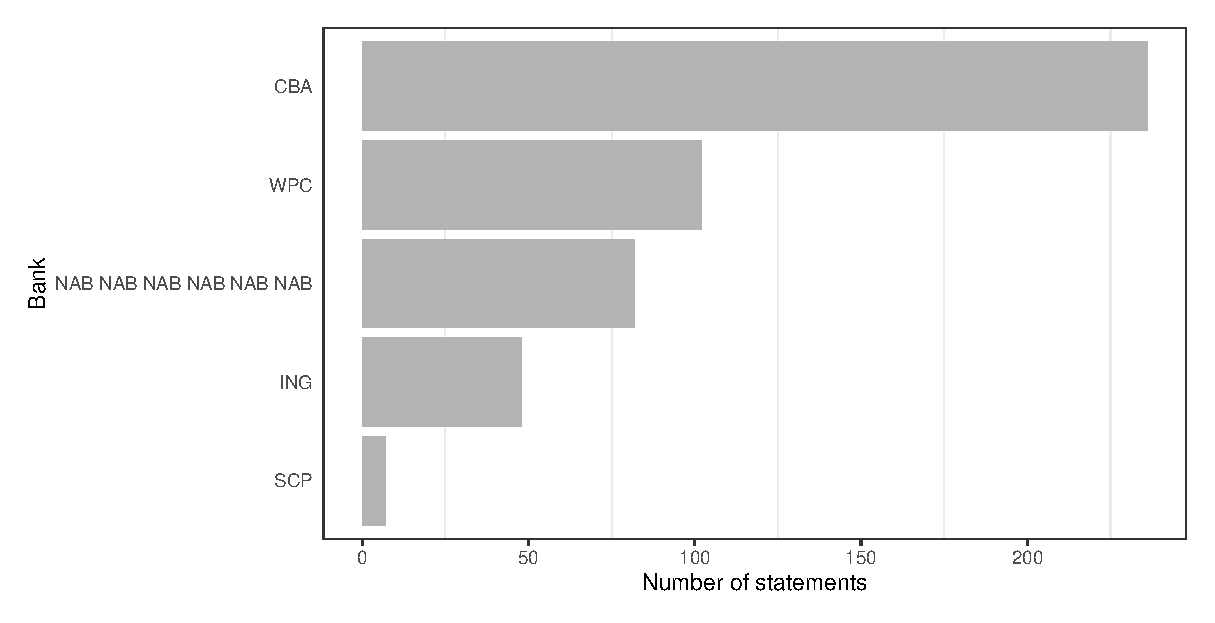
\includegraphics[width=0.75\textwidth]{banks}
\caption{The Distribution of Statements for Each Bank} \label{banks}
\end{figure}

\subsection{Experiment Design}
Each of the vectoriser is applied with each classifier, except Na\"ive Bayes which we could not use with Hashing, Google's Word2Vec and Doc2Vec vectoriser (because it is not compatible with them), making a total of 51 combinations to compare against our approach.

We have set aside 127 samples as test data while optimising the parameters using grid search. And used the remaining 348 to train models. We have ensured that for the minority classes, at least one sample remains in the training set. We have employed 10-fold cross validation (CV) techniques for the machine learning models and 3-fold CV for the deep learning models to select the best parameters using the training set. Table~\ref{parameters} shows all the parameter values used during the grid search. Once the best parameters are identified, we have induced a final model with the entire training set and evaluate the model on 127 test data.
\begin{table}[t]
\centering
\footnotesize
\caption{Parameters Used during Grid Search for Each Algorithm from Sci-kit Learn~\cite{scikit-learn} and Keras~\cite{chollet2015}}\label{parameters}
\begin{tabular}{ll}
\toprule
Algorithm & Parameters\\
\midrule
Frequency Vectoriser, & \texttt{ngram\_range}: [1, 4)\\
TF-IDF Vectoriser, & \texttt{max\_features}: [20, 40, 60, \ldots, 6800]\\
Hashing Vectoriser & \\
\midrule
GloVe, & \texttt{max\_features}: [20, 40, 60, \ldots, 6800]\\
Google's Word2Vec, & \\
Doc2Vec & \\
\midrule
Logistic Regression & \texttt{penalty}: \{none, $\ell_2$\}\\
& \texttt{C}: \{0.000001, 0.009, 0.001, 0.09, 0.01, 1, 5, 10, 25\}\\
& \texttt{max\_iter}: \{100, 120, 130, 140, 150\}\\
\midrule
Decision Tree & \texttt{criterion}: \{gini, entropy\}\\
& \texttt{min\_samples\_split}: \{2, 4, 5, 6\}\\
& \texttt{max\_features}: \{auto, sqrt, $\log$2, none\}\\
\midrule
Support Vector Machine & \texttt{C}: \{0.001, 0.01, 0.1, 1, 10, 100\}\\
& \texttt{kernel}: \{linear, poly, rbf, sigmoid\}\\
& \texttt{degree}: \{1, 2, 3\}\\
& \texttt{tol}: \{0.0001, 0.001, 0.1\}\\
& \texttt{decision\_function\_shape}: \{ovo, ovr\}\\ 
\midrule
Random Forest & \texttt{n\_estimators}: \{10, 11, 13, 15, 100, 115, 120, 125,\\
& 150, 200\}\\
& \texttt{criterion}: \{gini, entropy\}\\
& \texttt{min\_samples\_split}: \{2, 4, 5, 6\}\\
& \texttt{max\_features}: \{auto, sqrt, log2, None\}\\
\midrule
Na\"ive Bayes & \texttt{alpha}: \{0., 0.0001, 0.001, 0.01, 0.1, 1, 10\}\\
& \texttt{fit\_prior}: \{True, False\}\\
\midrule
$k$-Nearest Neighbour & \texttt{n\_neighbors}: \{3, 5, 7, 9, 11, 13\}\\
& \texttt{algorithm}: \{ball\_tree, kd\_tree, brute\}\\
& \texttt{leaf\_size}: \{30, 35, 30, 45, 50, 55\}\\
\midrule
Artificial Neural Network, & \texttt{activation}: \{relu, $\tanh$\}\\
CNN, & \texttt{optimizer}: \{SGD, Adam, Adamax, Adagrad,\\
LSTM-based RNN & Adadelta, Nadam, RMSprop\}\\
& \texttt{epochs}: \{10, 50, 100\}\\
& \texttt{learn\_rate}: \{0.01, 0.1, 0.2\}\\
\bottomrule
\end{tabular}
\end{table}

To test the effect of the size of the training set, we have also used 53 samples to train each model and used the remaining data to test the model performance. We then continue to add 59 samples to the training data and check the model performance on the remaining data. Eventually, we have trained each model with 53, 112, 171, 230, 289 and 348 training data and test the model performance on the remaining. 

\section{Results}\label{result}
Figure~\ref{resultset} shows the results for different algorithms used with different vectorisation methods while the size of the training data is growing. 
\begin{figure}[t]
%\footnotesize
\psfrag{CM2}[l][l][0.75]{CM$^2$}
\psfrag{TFVECT TFVECT TFVECT TFVECT}[l][l][0.6]{Term Frequency Vectoriser}
\psfrag{TFIDFVECT TFIDFVECT}[l][l][0.6]{TF$-$IDF Vectoriser}
\psfrag{HASHINGVECT HASHINGVECT}[l][l][0.6]{Hashing Vectoriser}
\psfrag{GLOETFIDFVECT GLOETFIDFVECT GL}[l][l][0.59]{GloVe with TF$-$IDF Vectoriser}
\psfrag{GOOGLEORD2VEC}[l][l][0.6]{Google's Word2Vec}
\psfrag{DOC2VEC}[l][l][0.6]{Doc2Vec}
\psfrag{VECT}[r][][0.85]{Vectoriser}
\psfrag{FMEASURE}[][][0.85]{$F$-measure (\%)}
\psfrag{SIZE OF TRAINING}[t][][0.85]{Size of Training Data Set}
\psfrag{LR}[][][0.65]{Logistic Regression}
\psfrag{DT}[][][0.65]{Decision Tree}
\psfrag{SVM}[][][0.65]{Support Vector Machine}
\psfrag{RF}[][][0.65]{Random Forest}
\psfrag{NB}[][][0.65]{Na\"ive Bayes}
\psfrag{KNN}[][][0.65]{k-Nearest Neighbour}
\psfrag{ANN}[][][0.65]{Artificial Neural Network}
\psfrag{CNN}[][][0.65]{Convolutional Neural Network}
\psfrag{LSTM}[][][0.65]{LSTM-based Recurrent Neural Network}
\psfrag{348}[b][][0.63]{348}
\psfrag{289}[b][][0.63]{289}
\psfrag{230}[b][][0.63]{230}
\psfrag{171}[b][][0.63]{171}
\psfrag{112}[b][][0.63]{112}
\psfrag{53}[b][][0.63]{53}
\psfrag{0.00}[r][r][0.65]{0}
\psfrag{0.25}[r][r][0.65]{25}
\psfrag{0.50}[r][r][0.65]{50}
\psfrag{0.75}[r][r][0.65]{75}
\psfrag{1.00}[r][r][0.65]{100}
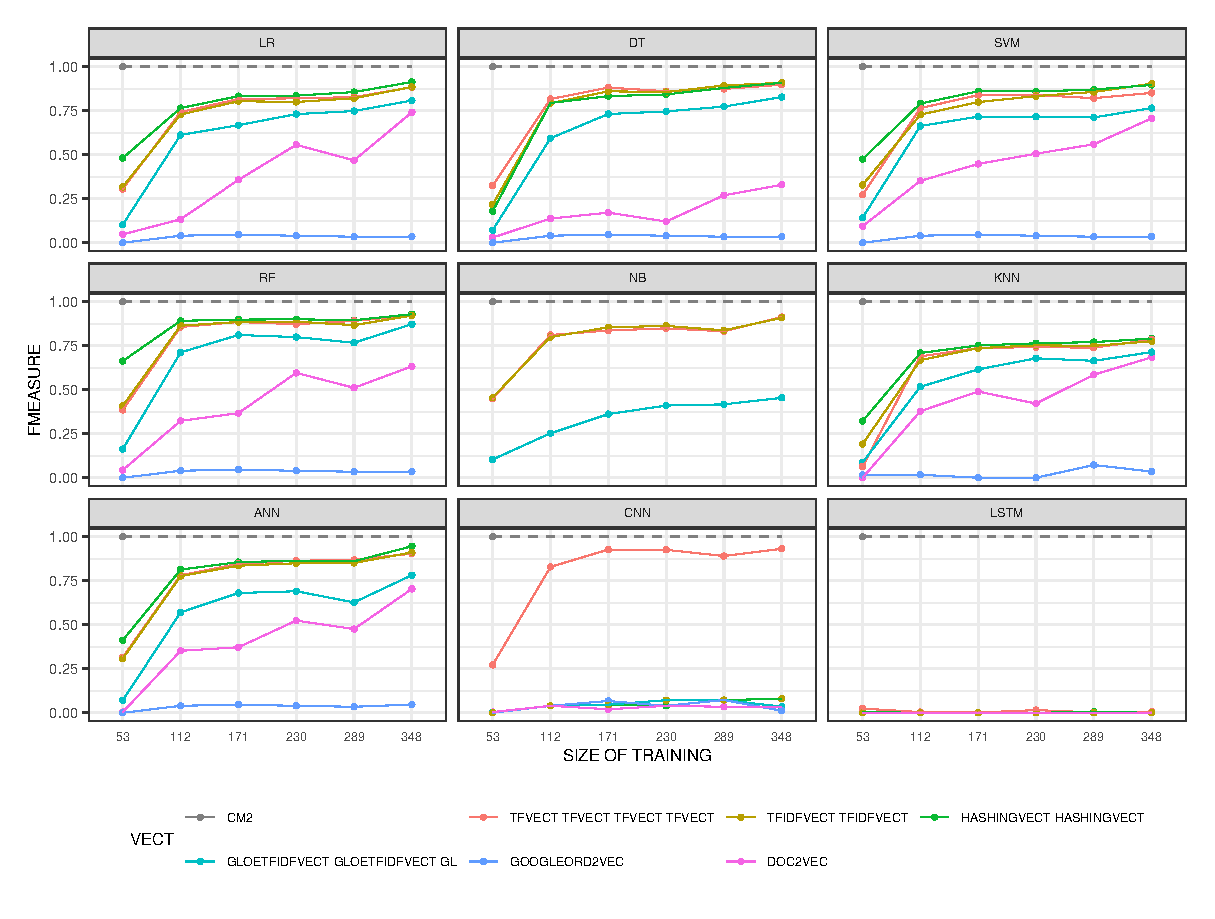
\includegraphics[width=\textwidth]{results}
\caption{Performance of Different Vectoriser with Every Classifier Compared Against CM$^2$ for Varying Training Data Set}\label{resultset}
\end{figure}
Each chart belongs to one machine learning approach and the colours denote the vectorisation method. As expected, the line charts show upward trends which indicates that the performance improves with the increased number of the training samples. This upward trend also demonstrates the trade-off between having the labelled data and the performance.

On average, Hashing Vectoriser performs better with most classifiers compared to other vectorisation methods especially for when using a smaller training data. Google's Word2Vec has the worst performance with any selected classifier. This is primarily because of banks sometimes use non-standard abbreviations in the transaction descriptions to fit larger words in a fixed-width text field and Google's pre-trained model is not designed for this type of situation.

The ensemble classifier Random Forest outperforms all other classification techniques, closely followed by a simple ANN. While LSTM performed very poorly due to the fact that it relies on very large training data and word sequence. In our experiment, LSTM had a training accuracy over 98\% when 348 documents have been used for training, but the model struggles to correctly identify more than 2 samples during testing.  Furthermore, bank statements do not really contain any sentences by which techniques like LSTM could benefit.
 
For this experiment, we run our algorithm only once as we only use 53 samples, and the result is shown with a grey dashed line in the charts. As we can see, our method outperforms all the machine learning methods regardless of the type of the classifier and vectoriser and the size of training data. It should be noted that all of the other models run with the best parameters we obtained from the grid searches. Though we have reported the best performances of these models using the best parameters, our algorithm still yields a better performance with a simple setting and the smallest set of training data. This shows considering the right features and designing a right approach is more important than switching or ensembling models.

Figure~\ref{penalty} shows the parameter sensitivity analysis for the maximum penalty, which is the only parameter required by our algorithm.
\begin{figure}
\centering
\psfrag{MAX}[t][][1]{Maximum Penalty}
\psfrag{FMEASURE}[b][][1]{$F$-measure (\%)}
\psfrag{500}[][][0.65]{500}
\psfrag{400}[][][0.65]{400}
\psfrag{300}[][][0.65]{300}
\psfrag{200}[][][0.65]{200}
\psfrag{100}[][][0.65]{100}
\psfrag{90}[r][r][0.65]{90}
\psfrag{92}[r][r][0.65]{92}
\psfrag{94}[r][r][0.65]{94}
\psfrag{96}[r][r][0.65]{96}
\psfrag{98}[r][r][0.65]{98}
\psfrag{10}[r][r][0.65]{100}
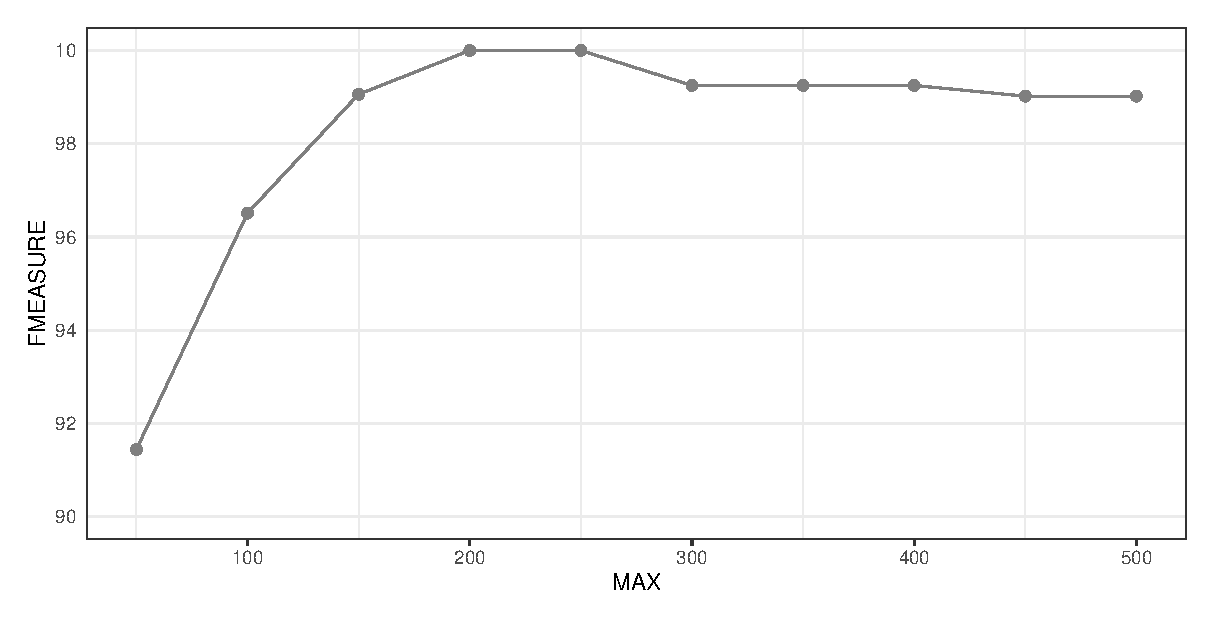
\includegraphics[width=0.75\textwidth]{penalty}
\caption{Effect of Different Maximum Penalty on CM$^2$ Performance}\label{penalty}
\end{figure}
We can see that for very small value the performance is lower because, our approach is quite sensitive to the coordinates of the keywords. In other words, if the keyword is just a little shifted from its expected position, we assume the keyword is not found. In practice, the location of the keywords may change because of scanning or having extra lines or space. At \texttt{maximum\_penalty} = 200, the accuracy is 100\%. Let us consider the resolution of an input image 2480 $\times$ 3500. If the keyword is around 10\% of the width apart from the original location of the keyword, it is considered as not found.

By increasing the maximum penalty more than 250, we also see a drop in accuracy because the keywords that are relatively far from each other are now considered matched. After 400, we do not see much difference in performance. The reason is when we put a very high threshold, only a few distances fall below the threshold. Theoretically, all the Manhattan distances in a 2480 $\times$ 3500 document is less than 2480 + 3500. Therefore, setting a threshold higher than 2480 + 3500 is useless and has no effect.

\section{Discussion}\label{discuss}
We have demonstrated how a human-level concept learning, when designed the right way, is far superior than machine learning methods especially when learning from limited data. In contrast to machine learning methods, which need hundreds of samples for each class to learn the concept, our approach needs only one sample and use the concept in a richer way. Just like human, our approach tries to match the test case to each of the known samples, estimates the similarities, and chooses the most similar class. Taking a deeper look, our approach finds the keywords and matches the keywords between the documents. However, if the matched keywords are too far from each other, it discards the matching and assumes there is no match for that keyword. Similarly, as a human, if we want to match the keywords to detect a document type, we would not match the keywords that are too far.
 
Another advantage of the human-level concept learning is the way we set the parameter. In a human-level concept learning, our understanding of the problem helps us to define the values for the algorithm parameters while for machine learning approaches, a parameter optimisation technique (i.e., grid search) needs to be used to find the best value. This can be very time consuming, and depends on how many parameters needs to be tuned, how many values to consider for each parameter or the computational complexity of the algorithm. Furthermore, the algorithm needs to run for each combination of the parameter setting. Still then, there is no guarantee that the best parameter value is amongst the considered parameter values.

When we want to set a value for \textit{maximum penalty}, we should ask ourselves this question ``what is the maximum distance that we want allow to match keywords?'' or ``how far a keyword can shift due to some extra line or extra space in a document?''. By looking at some sample documents, we estimate that $200$ is an appropriate value for the \textit{maximum penalty}. Definitely, it is better to check the other values but we expect the best value to be around $200$. On the other hand, assume we are using a deep learning model and we want to set values for $\ell_1$ and $\ell_2$. It is very hard to understand what these values actually mean for our problem. Therefore, we have to choose them by trial and error or by using grid search. In most cases, grid search with higher number of parameters results in overfitting~\cite{cawley2010}.
 
Designing a human-level concept learning starts with thinking about the way human does the job. First we look at the data, and then we should ask ourselves as human how do we solve the challenge. How do we recognise a template for bank statements where the contents are almost similar? The answer to the question identifies what feature to be used and how to design the approach.

\section{Conclusion}\label{conc}
Considering the way human learns, we developed a novel algorithm for classifying structured documents with similar content. The main strategy for us to design the algorithm was augmenting human intelligence to achieve a higher performance for our data. Unlike other typical machine learning algorithms that act mostly like a black-box, our approach encorporated the way we classify this type of documents in real life.

Human-level concept learning is not limited to only document classification or character recognition. The pain of providing the labelled data is obvious to industry regardless of the types of problems. This motivates us to deploy human-level concept learning approaches in various problem. As this model uses the distance of the keywords to identify similarity, in future, we would extend on this feature to extract entities relevant to the keywords from the structured documents.

\section*{Acknowledgement}
The authors thank ANZ Document, Knowledge and Content Automation team for providing the statements in PDFs and running through OCR to produce XML to conduct this research.


%
% ---- Bibliography ----
%
% BibTeX users should specify bibliography style 'splncs04'.
% References will then be sorted and formatted in the correct style.
%
% \bibliographystyle{splncs04}
% \bibliography{mybibliography}
%
\bibliographystyle{splncs04}
\bibliography{cm2.bib}{}
\end{document}
